\documentclass{beamer}
\usepackage[cefet,pt]{collegeBeamer}
\usepackage{xeCJK}
\usepackage{subfigure}

\definecolor{hrefcol}{RGB}{0, 0, 255} 

\title{Utilização de redes adversárias geradoras para super-resolução de imagens científicas}
\subtitle{Um estudo de caso}
\author{\href{mailto:leonam.teixeira.vasconcelos@gmail.com}{Leonam T. Vasconcelos}}
\date{Timóteo, 14 de Julho de 2025}

\begin{document}


    \maketitle

    \section{Introdução}


    \begin{frame}{Contexto}{\thesection \, \secname}
        \begin{itemize}
            \item Uma quantidade muito grande de imagens é produzida a todo momento do nosso cotidiano
                
                \begin{itemize}
                    \item Em média, o ser humano produziu cerca de 1,7 MB de dados por minuto no ano de  2020 \cite{vish_how_2020}
                \end{itemize}

            \item Esta taxa tende a apenas aumentar \cite{vish_how_2020}.
        \end{itemize}
    \end{frame}

    \begin{frame}{Motivação e Justificativa}{\thesection \, \secname}
        \begin{itemize}
            \item E se pudéssemos comprimir tais imagens, para reduzir os impactos desta enorme quantidade e depois, houvesse uma forma de recuperar a imagem original a partir da versão comprimida?

            \item Tal solução ainda poderia ser utilizada para recuperar detalhes de imagens originalmente em baixa resolução, como por exemplo:

            \begin{itemize}
                \item imagens médicas

                \item imagens científicas
            \end{itemize}
        \end{itemize}
    \end{frame}

    \begin{frame}{Motivação e Justificativa}{\thesection \, \secname}
        \begin{itemize}
            \item Estes dois grupos de imagens são particularmente interessantes, pois:
            \begin{enumerate}
                \item Imagens científicas, mais especificamente astronômicas de baixa resolução são facilmente encontradas online

                \item Algumas imagens médicas em particular como Ressonância Magnética não podem, em alguns casos, ser obtidas com uma qualidade maior devido à consequências à saúde do paciente exposto ao equipamento \cite{gupta_super-resolution_2020}
            \end{enumerate}
        \end{itemize}
    \end{frame}

    \begin{frame}{Objetivo Geral}{\thesection \, \secname}
        Experimentar os trabalhos de Ledig, Moreira e Wang  \cite{ledig_photo-realistic_2017, moreira_geracao_2019, wang_esrgan_2018} para a elaboração de redes adversárias geradoras treinadas especificamente para a super-resolução de imagens científicas a fim de validarmos os custos e benefícios deste treinamento específico em relação à modelos genericamente treinados.
    \end{frame}
    
    \begin{frame}{Objetivos específicos}{\thesection \, \secname}
        \begin{enumerate}
            \item Definir um sub-conjunto de imagens, especificamente de uma ou duas áreas para especializarmos o trabalho
        
            \item Definir um modelo de redes geradoras adversárias para o contexto apresentado
        	
            \item Integrar todo software e dependência necessários para treinar e utilizar o modelo escolhido no objetivo anterior
            
            \item Utilizar as bases de imagens para treinar o modelo escolhido de forma específica
        
            \item Utilizar-se de técnicas de cálculo de similaridade de imagens para avaliar o desempenho do treinamento realizado
        \end{enumerate}
    \end{frame}

    \section{Considerações preliminares}

    \begin{frame}{Sobre os requisitos teóricos}{\thesection \, \secname}

        Este trabalho se baseia fortemente em conceitos de redes neurais em diversas arquiteturas diferentes. Estas, estão mais profundamente detalhadas na monografia, deixando para esta apresentação, a retidão para com o tema.
        
    \end{frame}

    \begin{frame}{Sobre os requisitos teóricos | GAN}{\thesection \, \secname}

        \centering
        \includegraphics[width=9cm]{img/GAN_2.png} \\
        \label{fig:gan}
        \legend{RAG/GAN. Fonte: autor, baseado em \cite{gulli_deep_2019, zhang_dive_2021, moreira_geracao_2019}.}
        
    \end{frame}

    \begin{frame}{Sobre os requisitos teóricos | ESRGAN}{\thesection \, \secname}

        \centering
        \includegraphics[width=9cm]{img/SRGAN.png}\\
        \legend{SRGAN. Fonte: \cite{ledig_photo-realistic_2017}}
        
    \end{frame}

    \section{Procedimentos}

    \begin{frame}{Considerações sobre o fluxo de trabalho}{\thesection \, \secname}
        \begin{itemize}
            \item O desenvolvimento do trabalho foi dividido em 8 fases
            \item Algumas fases foram executadas uma única vez
            \item Outras, foram executadas em várias iterações
        \end{itemize}
    \end{frame}

    \begin{frame}{Detalhamento do fluxo de trabalho}{\thesection \, \secname}
        \centering
        \includegraphics[width=7cm]{img/flow_diagram_development.png} 
        \label{fig:diagrama_1}
    \end{frame}
    
    \begin{frame}{Detalhamento do fluxo de trabalho}{\thesection \, \secname}
        \centering
        \includegraphics[width=10cm]{img/flow_diagram_development_p1.png} \\
        \label{fig:diagrama_1}
    \end{frame}
    
    \begin{frame}{Detalhamento do fluxo de trabalho}{\thesection \, \secname}
        \centering
        \includegraphics[width=10cm]{img/flow_diagram_development_p2.png} \\
        \label{fig:diagrama_2}
    \end{frame}
    
    \begin{frame}{Detalhamento do fluxo de trabalho}{\thesection \, \secname}
        \centering
        \includegraphics[width=10cm]{img/flow_diagram_development_p3.png} \\
        \label{fig:diagrama_3}
    \end{frame}
    
    \section{Desenvolvimento}

    \begin{frame}{Captura de imagens para treinamento}{\thesection \, \secname \\ \textbf{\textit{Imagens astronômicas}}}

        As imagens astronômicas foram baixadas no site \textit{Kaggle} \cite{srivastava_astronomy_2024}

        \vspace{0.3cm}

        Exemplos:

        \centering

        \begin{figure}
            \subfigure{\includegraphics[width = 0.8cm]{img/astronomy-ds/1.jpg}} 
            \subfigure{\includegraphics[width = 0.8cm]{img/astronomy-ds/2.jpg}} 
            \subfigure{\includegraphics[width = 0.8cm]{img/astronomy-ds/3.jpg}} 
            \subfigure{\includegraphics[width = 0.8cm]{img/astronomy-ds/4.jpg}} 
            \subfigure{\includegraphics[width = 0.8cm]{img/astronomy-ds/5.jpg}}\\
            \subfigure{\includegraphics[width = 0.8cm]{img/astronomy-ds/6.jpg}} 
            \subfigure{\includegraphics[width = 0.8cm]{img/astronomy-ds/7.jpg}} 
            \subfigure{\includegraphics[width = 0.8cm]{img/astronomy-ds/8.jpg}} 
            \subfigure{\includegraphics[width = 0.8cm]{img/astronomy-ds/9.jpg}} 
            \subfigure{\includegraphics[width = 0.8cm]{img/astronomy-ds/10.jpg}}\\
            \subfigure{\includegraphics[width = 0.8cm]{img/astronomy-ds/11.jpg}} 
            \subfigure{\includegraphics[width = 0.8cm]{img/astronomy-ds/12.jpg}} 
            \subfigure{\includegraphics[width = 0.8cm]{img/astronomy-ds/13.jpg}} 
            \subfigure{\includegraphics[width = 0.8cm]{img/astronomy-ds/14.jpg}} 
            \subfigure{\includegraphics[width = 0.8cm]{img/astronomy-ds/15.jpg}}
        \end{figure} \\

        \legend{Fonte: Autor, com imagens do \textit{Kaggle} \cite{srivastava_astronomy_2024}.}

    \end{frame}

    \begin{frame}{Captura de imagens para treinamento}{\thesection \, \secname \\ \textbf{\textit{Imagens de ressonância magnética}}}

        As imagens de ressonância magnética foram encontradas em um repositório chamado \textit{Cancer Image Archive} \cite{cancer_imaging_archive_cancer_2022}.

        \vspace{0.2cm}
        
        \centering
        \includegraphics[width=6cm]{img/cancer_imaging_archive.png} \\
        \legend{Fonte: \textit{Cancer Image Archive} \cite{cancer_imaging_archive_cancer_2022}}

    \end{frame}
    
    \begin{frame}{Captura de imagens para treinamento}{\thesection \, \secname \\ \textbf{\textit{Imagens de ressonância magnética}}}

        Para fazer o \textit{download}, um instalador chamado \textit{NBIA Data Retriever} \cite{cancer_imaging_archive_cancer_2022} deve ser utilizado

        \vspace{0.2cm}

        \centering
        \includegraphics[width=6cm]{img/nbia_data_retriever.png} \\
        \legend{Fonte: Captura de tela tirada pelo autor.}

    \end{frame}
    
    \begin{frame}{Captura de imagens para treinamento}{\thesection \, \secname \\ \textbf{\textit{Imagens de ressonância magnética}}}

        Exemplos:

        \centering

        \begin{figure}
            \subfigure{\includegraphics[width=0.9cm]{img/mri-ds/1.png}} 
            \subfigure{\includegraphics[width=0.9cm]{img/mri-ds/2.png}} 
            \subfigure{\includegraphics[width=0.9cm]{img/mri-ds/3.png}} 
            \subfigure{\includegraphics[width=0.9cm]{img/mri-ds/4.png}} 
            \subfigure{\includegraphics[width=0.9cm]{img/mri-ds/5.png}}\\
            \subfigure{\includegraphics[width=0.9cm]{img/mri-ds/6.png}} 
            \subfigure{\includegraphics[width=0.9cm]{img/mri-ds/7.png}} 
            \subfigure{\includegraphics[width=0.9cm]{img/mri-ds/8.png}} 
            \subfigure{\includegraphics[width=0.9cm]{img/mri-ds/9.png}} 
            \subfigure{\includegraphics[width=0.9cm]{img/mri-ds/10.png}}\\
            \subfigure{\includegraphics[width=0.9cm]{img/mri-ds/11.png}} 
            \subfigure{\includegraphics[width=0.9cm]{img/mri-ds/12.png}} 
            \subfigure{\includegraphics[width=0.9cm]{img/mri-ds/13.png}} 
            \subfigure{\includegraphics[width=0.9cm]{img/mri-ds/14.png}} 
            \subfigure{\includegraphics[width=0.9cm]{img/mri-ds/15.png}}
        \end{figure}

        \legend{Fonte: Autor, com imagens do \textit{Cancer Imaging Archive} \cite{cancer_imaging_archive_cancer_2022}.}

    \end{frame}

    \begin{frame}{Ajustes nas imagens médicas}{\thesection \, \secname}

        As imagens médicas são armazenadas e propagadas em um formato específico: DICOM. \cite{dicom_standard_history_2019, medical_connections_dicomobjects_2011, dicom_standard_current_2024, medical_connections_dicom_2007, weston_understanding_2020}

        \centering
        \includegraphics[width=6cm]{img/dicom_img.png} \\
        \legend{Estrutura de imagens \textit{DICOM}. Fonte: Autor.}

    \end{frame}

    \begin{frame}{Ajustes nas imagens médicas}{\thesection \, \secname}

        \centering
        \includegraphics[width=9cm]{img/number_of_frames.png}\\
        \legend{Destacando o número de frames -- ou número de imagens -- nos \\
                metadados de um arquivo \textit{DICOM}. Fonte: Autor.}

    \end{frame}

    \begin{frame}{Ajustes nas imagens médicas}{\thesection \, \secname}

        \centering
        \includegraphics[width=7cm]{img/code_2.png} \\
        \legend{Código para converter uma imagem \textit{DICOM} para o \\
                formato \textit{jpg}. Fonte: Autor.}

    \end{frame}

    \begin{frame}{Preparação das imagens para treinamento}{\thesection \, \secname}

        Como requisitos obrigatórios para o treinamento, as imagens devem estar em:

        \begin{itemize}
            \item resolução uniforme
            \item resolução divisível por 4 (específico ao problema atual)
            \item um formato compatível
            \item uma estrutura esperada pelo modelo
        \end{itemize}

    \end{frame}

    \begin{frame}{Preparação das imagens para treinamento}{\thesection \, \secname}

        O modelo espera que as imagens estejam distribuídas no formato a seguir:

        \begin{itemize}
            \item Treinamento
            \begin{itemize}
                \item HR
                \begin{itemize}
                    \item Imagens de treinamento com alta resolução
                \end{itemize}  

                \item LR 
                \begin{itemize}
                    \item Imagens de treinamento com baixa resolução (4x menor que HR)
                \end{itemize}        
            \end{itemize}        
            \item Validação
            \begin{itemize}
                \item HR
                \begin{itemize}
                    \item Imagens de validação com alta resolução 
                \end{itemize}        
                \item LR 
                \begin{itemize}
                    \item Imagens de validação com baixa resolução (4x menor que HR)
                \end{itemize}        
            \end{itemize}        
        \end{itemize}

    \end{frame}

    \begin{frame}{Preparação das imagens para treinamento}{\thesection \, \secname}

        \centering
        \includegraphics[width=06cm]{img/magick-utils.png} \\
        \legend{Captura de tela do software \textit{Magick-Utils}. \\ 
                Fonte: \textit{Github} do criador do software \cite{n00mkrad_magickutils_2022}.}

    \end{frame}

    
    
    \begin{frame}{Preparação do ambiente para treinamento}{\thesection \, \secname}

        Esta fase inclui:

        \begin{itemize}
            \item Instalação de dependências$^\ast$
            \begin{itemize}
                \item Drivers necessários
                \item Versão correta do \textbf{python}
                \item Dependências do modelo utilizado
            \end{itemize}
            \item Execução preliminar para checagem de consistência.
        \end{itemize}

    \end{frame}

    \begin{frame}{Preparação do ambiente para treinamento}{\thesection \, \secname}

        \centering
        \includegraphics[width=8cm]{img/version_diagram.png} \\
        \legend{Diagrama de interação entre as partes envolvidas \\
                no modelo. Fonte: Autor.}

    \end{frame}

    \begin{frame}{Treinamento}{\thesection \, \secname}
        
        \centering

        Descrição do hardware disponível:

        \vspace{0.2cm}

        \begin{tabular}{|l|l|} \hline
            \textbf{Item}            & \textbf{Descrição}                    \\ \hline
            CPU                      & Intel i7 Octa Core                    \\ \hline
            Memória RAM              & 16GB                                  \\ \hline
            Memória de Vídeo         & 2GB                                   \\ \hline
            Modelo da placa de vídeo & GeForce MX350                         \\ \hline
            Disco                    & 512GB (apenas 90GB disponível)        \\ \hline
            Sistema operacional      & Windows 10 e Ubuntu 24.04 disponíveis  \\ \hline
        \end{tabular}
        
    \end{frame}

    \begin{frame}{Treinamento}{\thesection \, \secname}
        
        \centering
        
        Parâmetros de treinemento:

        \vspace{0.2cm}

        \begin{tabular}{|l|l|} \hline
            \textbf{\textit{batch size}}         & 2    \\ \hline
            \textbf{Nº de épocas}                & 100  \\ \hline
            \textbf{Nº de interações por época}  & 1000 \\ \hline 
        \end{tabular}

    \end{frame}

    \begin{frame}{Coleta de dados}{\thesection \, \secname}

        \centering
        \begin{tabular}{c c c}
            \includegraphics[width=2.5cm]{img/samples/mri/mri_original.png}                 & 
            \includegraphics[width=2.5cm]{img/samples/mri/mri_non_specific_training.png}    & 
            \includegraphics[width=2.5cm]{img/samples/mri/mri_specific_training.png} \\
            (a) & (b) & (c)
        \end{tabular} \\
        \legend{Amostra aleatoriamente capturada das imagens de ressonância.\\
                Fonte: Autor}.

    \end{frame}

    \begin{frame}{Coleta de dados}{\thesection \, \secname}

        \centering
        \begin{tabular}{c c c}
            \includegraphics[width=2.5cm]{img/samples/astronomy/astronomy_original.png}              &
            \includegraphics[width=2.5cm]{img/samples/astronomy/astronomy_non_specific_training.png} & 
            \includegraphics[width=2.5cm]{img/samples/astronomy/astronomy_specific_training.png}     \\
            (a) & (b) & (c)
        \end{tabular} \\
        \legend{Amostra aleatoriamente capturada das imagens de astronomia.\\ Fonte: Autor}.

    \end{frame}

    \section{Resultados}

    \begin{frame}{Resultados: Ressonância Magnética}{\thesection \, \secname}

        \centering
        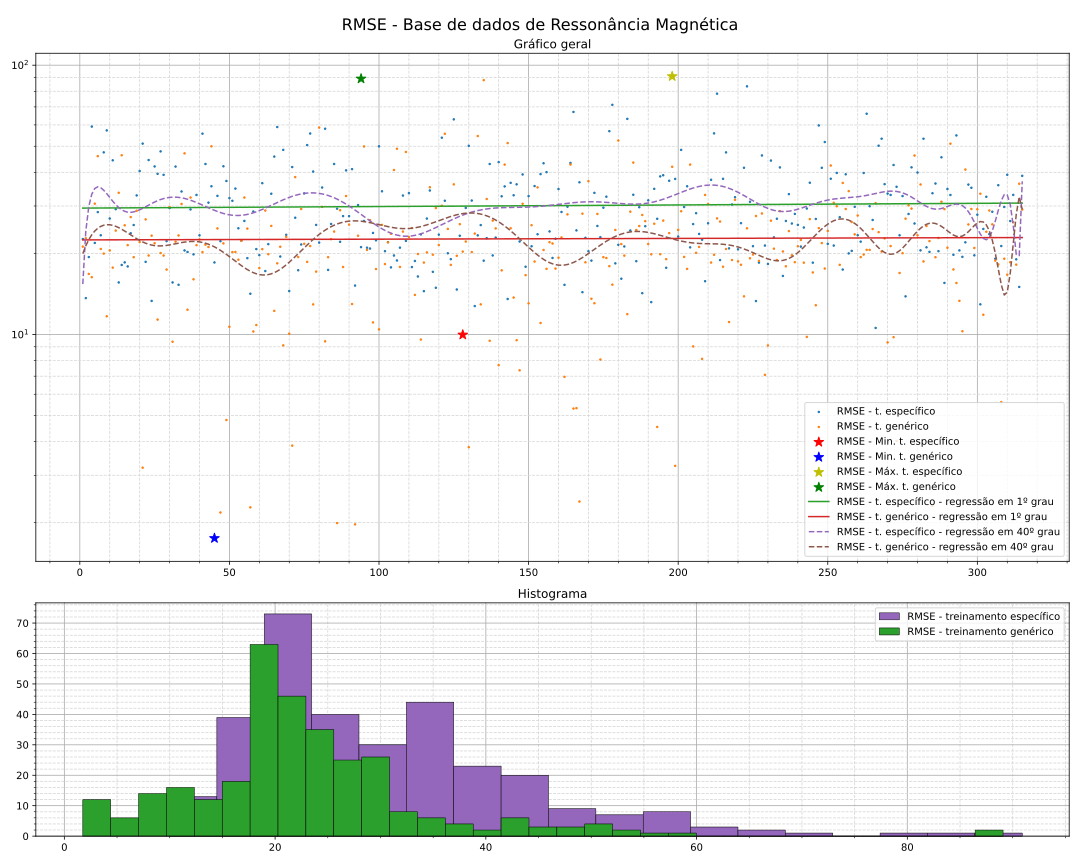
\includegraphics[width=7.5cm]{img/resultados/rmse_mri_compound.png} \\
        \legend{Cálculo de erro RMSE para base de dados de ressonância magnética. Fonte: Autor}.

    \end{frame}

    \begin{frame}{Resultados: Ressonância Magnética}{\thesection \, \secname}

        \centering
        \includegraphics[width=10.5cm]{img/resultados/rmse_mri_cropped.png} \\
        \legend{Gráfico de erro RMSE (ressonância) ampliado. Fonte: Autor}.

    \end{frame}

    \begin{frame}{Resultados: Astronomia}{\thesection \, \secname}
        
        \centering
        \includegraphics[width=7.5cm]{img/resultados/rmse_astronomy_compound.png} \\
        \legend{Cálculo de erro RMSE para base de dados astronômica. Fonte: Autor}.

    \end{frame}

    \begin{frame}{Resultados: Astronomia}{\thesection \, \secname}
        
        \centering
        \includegraphics[width=10.5cm]{img/resultados/rmse_astronomy_cropped.png} \\
        \legend{Gráfico de erro RMSE (astronomia) ampliado. Fonte: Autor}.

    \end{frame}

    \section{Conclusão}

    \begin{frame}{Conclusão}{\thesection \, \secname}
        
        O treinamento \textbf{genérico} produziu consistentemente, melhores resultados que os treinamentos \textbf{específicos}.

        \vspace{0.2cm}
        
        \pause

        Possíveis motivos:

        \begin{itemize}
            \item Limitações de recursos: memória e processador
            \pause 
            \item Limitação de tempo
        \end{itemize}

    \end{frame}

    \section{Referências}

    \begin{frame}[allowframebreaks]
        \bibliographystyle{abbrv}
        \bibliography{references}
    \end{frame}
\end{document}
